\chapter{Исследовательский раздел}
\label{cha:research}

\section{Пример работы}

\section{Технические характеристики}
\begin{itemize}
    \item Процессор: AMD Ryzen 2700 4.00GHz.[3]
    \item Оперативная память: 16GiB.
    \item Операционная система: Linux Kernel 5.14.8 [4].
\end{itemize}

\section{Время выполнения алгоритмов}

Время выполнения алгоритмов было найдено при помощи библиотеки Google Benchmark [5]. 
Результаты измерения времени (в наносекнудах) были зафиксированы в Таблице \ref{tab:benchmark}.

\begin{table}[ht]
  \caption{Замер времени для строк размером от 1 до 100. }
  \begin{tabular}{|c|c|c|c|c|}
  \hline
  Длина & Рекурсивный & Итеративный  & Кэшированный & Дамерау--Левенштейн \\
  \hline
  1  &  $6,383$   &  $20,485$   & 226,476 & 114,539            \\
    \hline
  2  & $9,821$   & $40,6785$    & 347,944 & 143,76        \\
    \hline
  3  & $13,153$   & $64,580$    & 210,886 & 204,811         \\
    \hline
  4  & $16,299$  & $97,210$   & 261,35  & 263,149 \\
    \hline
  5  &  $19,797$ & $180,148$   & 372,485  & 355,953       \\
  \hline
    10  &  $37,74$ &  $477,512$  & 766,765  & 1170,651     \\
      \hline
    20  &  $82,742$ &  $2096,517$  & 2275,018  & 4067,035  \\
  \hline
  50  &  $207,150$ &  $11792,425$  & 11844,141  & 25213,385 \\
  \hline
  100  &  $394,308$ &  $43001,695$  & 42887,397  & 99859,339   \\
  \hline
  \end{tabular}
  \label{tab:benchmark}
\end{table}

\begin{figure}
    \centering
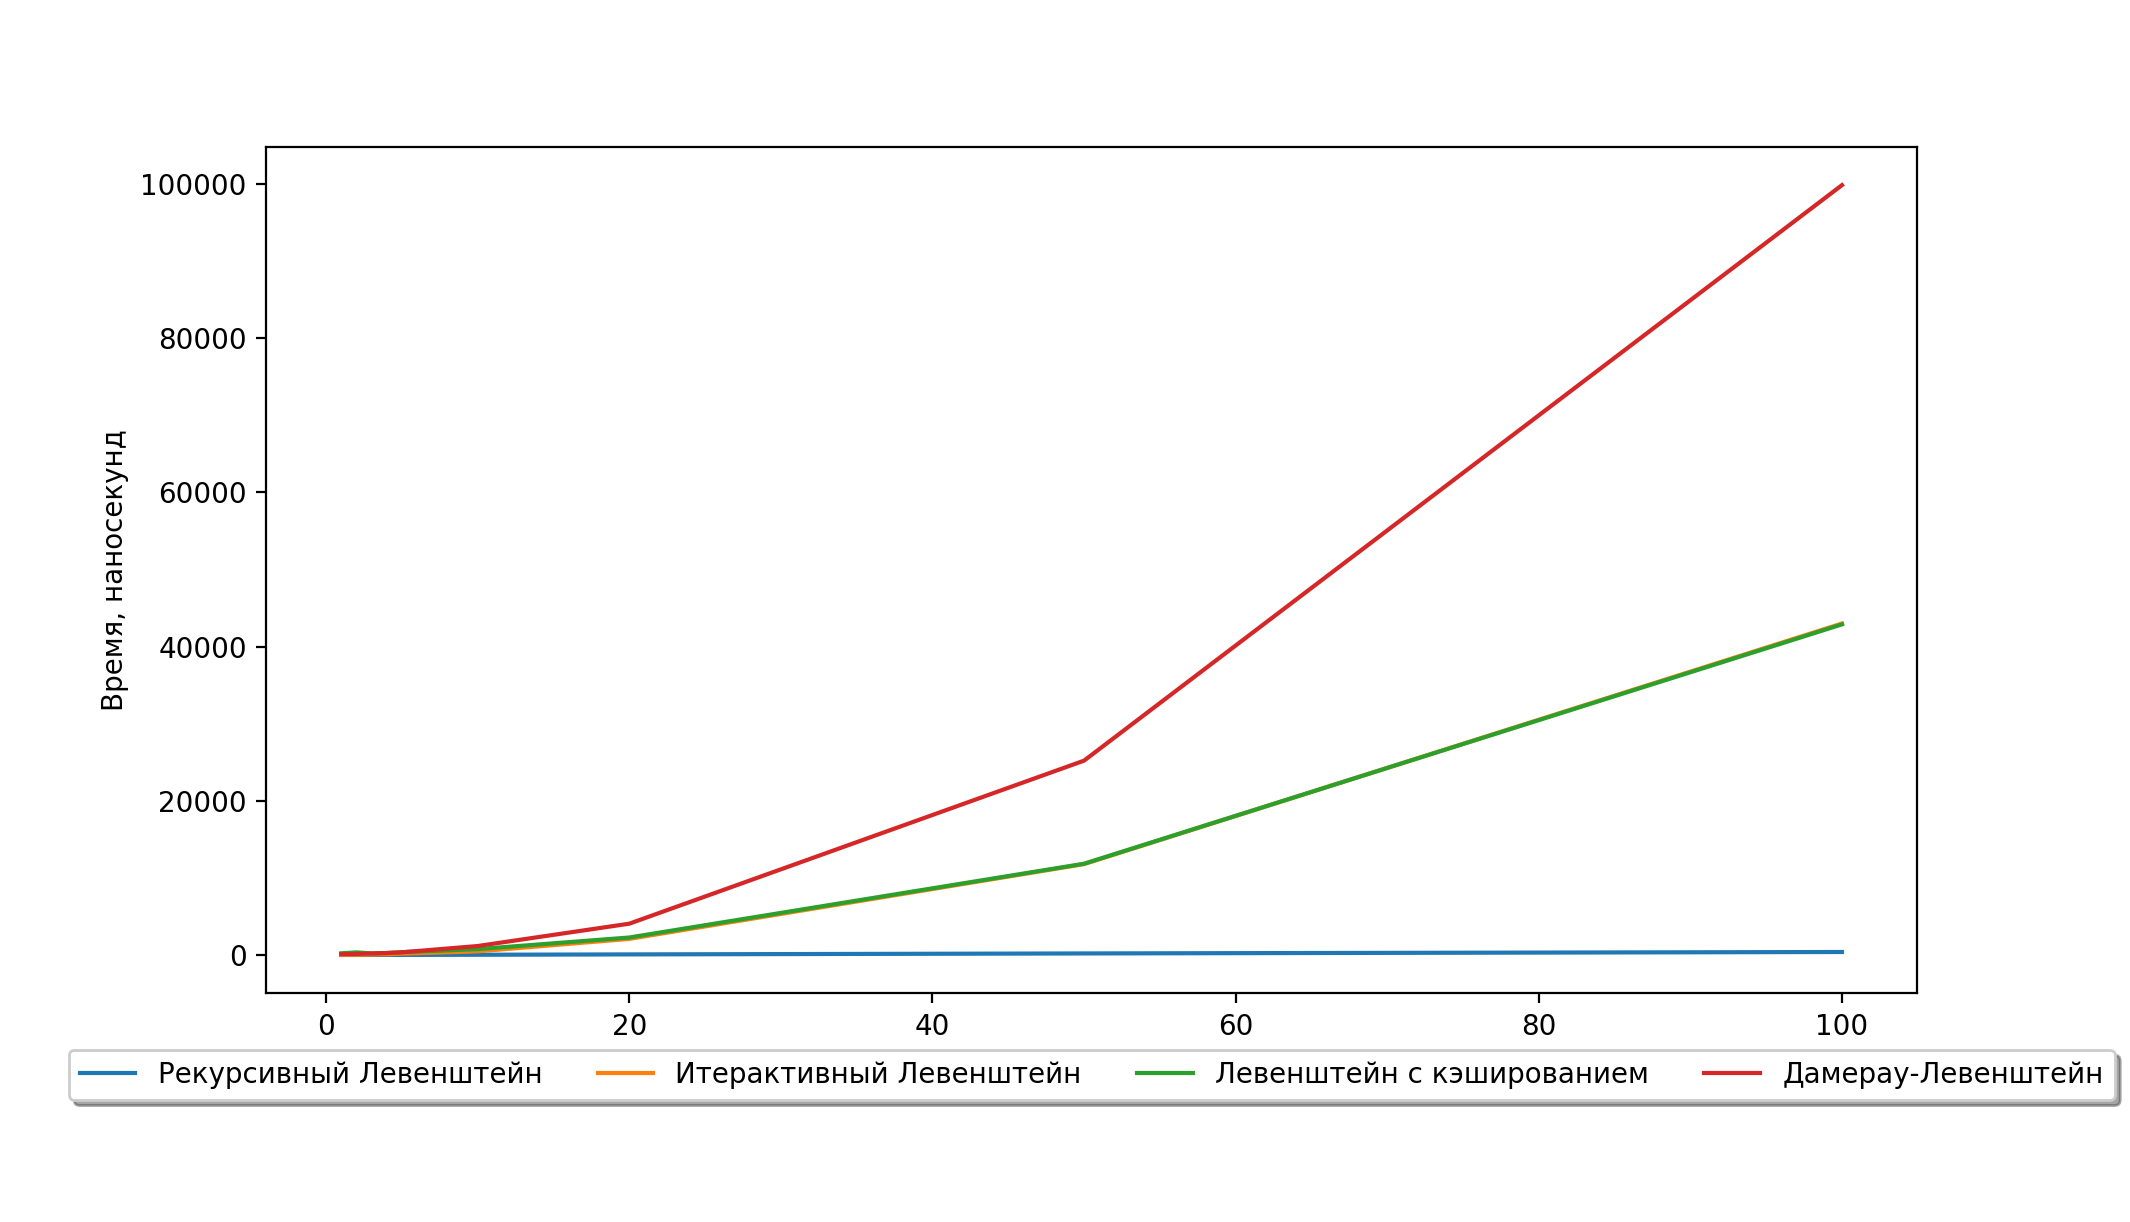
\includegraphics[width=\textwidth]{sem-v-aa-master/lab1/tex/inc/plots/Figure_1.png}

    \caption{Временные характеристики различных реализаций алгоритмов}
    \label{fig:timestamps}
\end{figure}

В диапазоне длины слова от 1 до 20 скорость работы различных алгоритмов разнится не более чем на порядок. При длине слова, превышающей 20 символов разница выполнения алгоритмов становится намного заметнее. Наиболее эффективным в показаном эксперименте оказался рекурсивный алгоритм Левенштейна, а менее всего -- Дамерау--Левенштейн. 
Из этого можно сделать вывод о эффективности вышеприведенных функций. Наиболее эффективной является итеративная реализация, опережающая на 3-5 порядков реализации рекурсивные и реализацию алгоритма Дамерау--Левенштейна. 

\section{Характеристика по памяти}

\par
	Алгоритмы Левенштейна и Дамерау-Левенштейна не отличаются по использованию памяти, соответственно достаточно рассмотреть рекурсивный и матричный реализации этих алгоритмов.
	\par
	Максимальная глубина стека вызовов при рекурсивной реализации равна сумме длин входящих строк, а на каждый вызов функции требуется еще 5 дополнительных переменных типа \textit{usize}, соответственно, максимальный расход памяти
	\begin{equation}
		(Size(S_{1}) + Size(S_{2}) \cdot (2 \cdot Size(\text{string}) + 5 \cdot Size(\text{usize})))
	\end{equation}
	
	\noindent
	где Size - функция, возвращающая размер аргумента; string - строковый тип, usize - целочисленный, беззнаковый тип.
	\par
	Использование памяти при итеративной реализации теоритически равно
	\begin{equation}
		\label{eq:mem_req}
		(Size(S_{1} + 1) \cdot Size(S_{2} + 1)) \cdot Size(usize) + 2 \cdot Size(string)
	\end{equation}
	\par
	Использование памяти рекурсивной реализации алгоритма Левенштейна с кэшем теоритически равно
	\begin{multline}
		\label{eq:mem_iter}
		(Size(S_{1}) + Size(S_{2}) \cdot (2 \cdot Size(string) +\\+ 5 \cdot Size(usize)) + (Size(S_{1} + 1) \cdot Size(S_{2} + 1)) \cdot Size(usize))
	\end{multline}

\begin{table}[ht]
  \caption{Замер памяти для строк размером от 1 до 100. }
  \begin{tabular}{|c|c|c|c|c|}
  \hline
  Длина & Рекурсивный & Итеративный  & Кэшированный & Дамерау--Левенштейн \\
  \hline
  1  &  $6,383$   &  $20,485$   & 226,476 & 114,539            \\
    \hline
  2  & $9,821$   & $40,6785$    & 347,944 & 143,76        \\
    \hline
  3  & $13,153$   & $64,580$    & 210,886 & 204,811         \\
    \hline
  4  & $16,299$  & $97,210$   & 261,35  & 263,149 \\
    \hline
  5  &  $19,797$ & $180,148$   & 372,485  & 355,953       \\
  \hline
    10  &  $37,74$ &  $477,512$  & 766,765  & 1170,651     \\
      \hline
    20  &  $82,742$ &  $2096,517$  & 2275,018  & 4067,035  \\
  \hline
  50  &  $207,150$ &  $11792,425$  & 11844,141  & 25213,385 \\
  \hline
  100  &  $394,308$ &  $43001,695$  & 42887,397  & 99859,339   \\
  \hline
  \end{tabular}
  \label{tab:memory}
\end{table}


\section{Вывод}

	\par
	Рекурсивный алгоритм Левенштейна работает на порядок дольше итеративных реализаций, время его работы увеличивается в геометрической прогрессии. На словах длиной 9 символов, матричная реализация превосходит рекурсивную в 4800 раз. Рекурсивные алгоритмы Левенштейна и Дамерау - Левенштейна сопостовимы по времени. Однако, использование кэша значительно ускоряет рекурсивный алгоритм, но он все еще не превосходит матричную реализацию.
	Из формул \ref{eq:mem_req}-\ref{eq:mem_iter} можно сделать вывод, что рекурсивные алгоритмы потребляют больше памяти, чем матричные, при одинаковых длин строк.

%%% Local Variables:
%%% mode: latex
%%% TeX-master: "rpz"
%%% End:
